\documentclass[12pt]{article} % 12pt 为字号大小 UTF8
\usepackage{amssymb,amsfonts,amsmath,amsthm}
%\usepackage{fontspec,xltxtra,xunicode}
%\usepackage{times}

%----------
% 定义中文环境
%----------

\usepackage{xeCJK}
\usepackage{caption}
\captionsetup{font={tiny}}%调整注释字体
\setCJKmainfont[BoldFont={SimHei},ItalicFont={KaiTi}]{SimSun}
\setCJKsansfont{SimHei}
\setCJKfamilyfont{zhsong}{SimSun}
\setCJKfamilyfont{zhhei}{SimHei}

\newcommand*{\songti}{\CJKfamily{zhsong}} % 宋体
\newcommand*{\heiti}{\CJKfamily{zhhei}}   % 黑体

%\textbf{}加粗字体
%----------
% 版面设置
%----------
%首段缩进
\usepackage{indentfirst}
\setlength{\parindent}{2.1em}
%\indent在每行前缩进
%行距
\renewcommand{\baselinestretch}{1.4} % 1.4倍行距

%页边距
\usepackage[a4paper]{geometry}
\geometry{verbose,
	tmargin=3cm,% 上边距
	bmargin=3cm,% 下边距
	lmargin=3cm,% 左边距
	rmargin=3cm % 右边距
}


%----------
% 其他宏包
\usepackage{listings}%插入代码
\usepackage{booktabs}%插入excel
\usepackage{adjustbox}
%----------
%图形相关
\usepackage[x11names]{xcolor} % must before tikz, x11names defines RoyalBlue3
\usepackage{graphicx}
\usepackage{pstricks,pst-plot,pst-eps}
\usepackage{subfig}
\def\pgfsysdriver{pgfsys-dvipdfmx.def} % put before tikz
\usepackage{tikz}

%原文照排
\usepackage{verbatim}

%网址
\usepackage{url}
\usepackage[framed,numbered,autolinebreaks,useliterate]{mcode}%代码高亮

%----------
% 习题与解答环境
%----------
% %习题环境
% \theoremstyle{definition} 
% \newtheorem{exs}{习题}

% %解答环境
% \ifx\proof\undefined\
% \newenvironment{proof}[1][\protect\proofname]{\par
% \normalfont\topsep6\p@\@plus6\p@\relax
% \trivlist
% \itemindent\parindent
% \item[\hskip\labelsep
% \scshape
% #1]\ignorespaces
% }{%
% \endtrivlist\@endpefalse
% }
% \fi

% \renewcommand{\proofname}{\it{证明}}

%----------
% 我的自定义
%----------

\newcommand{\horrule}[1]{\rule[0.5ex]{\linewidth}{#1}} 	% Horizontal rule

\renewcommand{\refname}{参考文献}
\renewcommand{\abstractname}{\large \bf 摘\quad 要}
\renewcommand{\contentsname}{目录}
\renewcommand{\tablename}{表}
\renewcommand{\figurename}{图}

\setlength{\parskip}{0.4ex} % 段落间距

\usepackage{enumitem}
\setenumerate[1]{itemsep=0pt,partopsep=0pt,parsep=\parskip,topsep=5pt}
\setitemize[1]{itemsep=0.4ex,partopsep=0.4ex,parsep=\parskip,topsep=0.4ex}
\setdescription{itemsep=0pt,partopsep=0pt,parsep=\parskip,topsep=5pt}


%==========
% 正文部分
%==========

\begin{document}
	\title{
		%	{\normalfont\normalsize\textsc{
		%			Xiangtan University  \\[25pt]}}
		\horrule{0.5pt}\\
		\sffamily{现实中的优化问题\\2004数学建模国赛B题第三问}
		\horrule{1.8pt}\\[20pt]
	}
	\author{米科润\quad 19信计二班\\201905755824}
	\date{\today} % 若不需要自动插入日期,则去掉前面的注释;{ } 中也可以自定义日期格式
	
	\begin{titlepage}
		\maketitle
		\vspace{30pt}
		\thispagestyle{empty}
	\end{titlepage}
	
	\tableofcontents
	\thispagestyle{empty}
	
	\newpage
	\setcounter{page}{1}
	
	\section{Background and Problem}
	电力从生产到使用的四大环节——发电、输电、配电和用电是瞬间完成的。我国电力市场初期是发电侧电力市场,采取交易与调度一体化的模式。电网公司在组织交易、调度和配送时,必须遵循电网“安全第一”的原则,同时要制订一个电力市场交易规则,按照购电费用最小的经济目标来运作。市场交易-调度中心根据负荷预报和交易规则制订满足电网安全运行的调度计划――各发电机组的出力(发电功率)分配方案;在执行调度计划的过程中,还需实时调度承担AGC(自动发电控制)辅助服务的机组出力,以跟踪电网中实时变化的负荷。\\
	设某电网有若干台发电机组和若干条主要线路,每条线路上的有功潮流(输电功率和方向)取决于电网结构和各发电机组的出力。电网每条线路上的有功潮流的绝对值有一安全限值,限值还具有一定的相对安全裕度(即在应急情况下潮流绝对值可以超过限值的百分比的上限)。如果各机组出力分配方案使某条线路上的有功潮流的绝对值超出限值,称为输电阻塞。当发生输电阻塞时,需要研究如何制订既安全又经济的调度计划。\\
	\indent 电力市场交易规则:\\
	\indent 1. 以15分钟为一个时段组织交易,每台机组在当前时段开始时刻前给出下一个时段的报价。各机组将可用出力由低到高分成至多10段报价,每个段的长度称为段容量,每个段容量报一个价(称为段价),段价按段序数单调不减。在最低技术出力以下的报价一般为负值,表示愿意付费维持发电以避免停机带来更大的损失。\\
	\indent 2. 在当前时段内,市场交易-调度中心根据下一个时段的负荷预报,每台机组的报价、当前出力和出力改变速率,按段价从低到高选取各机组的段容量或其部分(见下面注释),直到它们之和等于预报的负荷,这时每个机组被选入的段容量或其部分之和形成该时段该机组的出力分配预案(初始交易结果)。最后一个被选入的段价(最高段价)称为该时段的清算价,该时段全部机组的所有出力均按清算价结算。\\
	\indent 注释:\\
	\indent (a)	每个时段的负荷预报和机组出力分配计划的参照时刻均为该时段结束时刻。\\
	\indent (b)机组当前出力是对机组在当前时段结束时刻实际出力的预测值。\\
	\indent (c)假设每台机组单位时间内能增加或减少的出力相同,该出力值称为该机组的爬坡速率。由于机组爬坡速率的约束,可能导致选取它的某个段容量的部分。\\
	\indent (d)为了使得各机组计划出力之和等于预报的负荷需求,清算价对应的段容量可能只选取部分。\\
	\indent \textbf{你需要做的工作如下:}\\
	\indent 假设下一个时段预报的负荷需求是982.4MW,表3、表4和表5分别给出了各机组的段容量、段价和爬坡速率的数据,试按照电力市场规则给出下一个时段各机组的出力分配预案。\\

	
	
	\section{Data}
		\begin{table}[htbp]
		\centering
		\caption{各机组段容量}
		\resizebox{\textwidth}{30mm}{
		\begin{tabular}{|c|r|r|r|r|r|r|r|r|r|r|}
			\toprule
			机组\textbackslash{}段 & \multicolumn{1}{c|}{1} & \multicolumn{1}{c|}{2} & \multicolumn{1}{c|}{3} & \multicolumn{1}{c|}{4} & \multicolumn{1}{c|}{5} & \multicolumn{1}{c|}{6} & \multicolumn{1}{c|}{7} & \multicolumn{1}{c|}{8} & \multicolumn{1}{c|}{9} & \multicolumn{1}{c|}{10} \\
			\midrule
			1     & 70    & 0     & 50    & 0     & 0     & 30    & 0     & 0     & 0     & 40 \\
			\midrule
			2     & 30    & 0     & 20    & 8     & 15    & 6     & 2     & 0     & 0     & 8 \\
			\midrule
			3     & 110   & 0     & 40    & 0     & 30    & 0     & 20    & 40    & 0     & 40 \\
			\midrule
			4     & 55    & 5     & 10    & 10    & 10    & 10    & 15    & 0     & 0     & 1 \\
			\midrule
			5     & 75    & 5     & 15    & 0     & 15    & 15    & 0     & 10    & 10    & 10 \\
			\midrule
			6     & 95    & 0     & 10    & 20    & 0     & 15    & 10    & 20    & 0     & 10 \\
			\midrule
			7     & 50    & 15    & 5     & 15    & 10    & 10    & 5     & 10    & 3     & 2 \\
			\midrule
			8     & 70    & 0     & 20    & 0     & 20    & 0     & 20    & 10    & 15    & 5 \\
			\bottomrule
		\end{tabular}}
		\label{tab:addlabel}%
			\centering
		\caption{各机组段价}
		\resizebox{\textwidth}{30mm}{
\begin{tabular}{|r|r|r|r|r|r|r|r|r|r|r|}
	\toprule
	\multicolumn{1}{|l|}{机组\textbackslash{}段} & \multicolumn{1}{c|}{1} & \multicolumn{1}{c|}{2} & \multicolumn{1}{c|}{3} & \multicolumn{1}{c|}{4} & \multicolumn{1}{c|}{5} & \multicolumn{1}{c|}{6} & \multicolumn{1}{c|}{7} & \multicolumn{1}{c|}{8} & \multicolumn{1}{c|}{9} & \multicolumn{1}{c|}{10} \\
	\midrule
	1     & -505  & 0     & 124   & 168   & 210   & 252   & 312   & 330   & 363   & 489 \\
	\midrule
	2     & -560  & 0     & 182   & 203   & 245   & 300   & 320   & 360   & 410   & 495 \\
	\midrule
	3     & -610  & 0     & 152   & 189   & 233   & 258   & 308   & 356   & 415   & 500 \\
	\midrule
	4     & -500  & 150   & 170   & 200   & 255   & 302   & 325   & 380   & 435   & 800 \\
	\midrule
	5     & -590  & 0     & 116   & 146   & 188   & 215   & 250   & 310   & 396   & 510 \\
	\midrule
	6     & -607  & 0     & 159   & 173   & 205   & 252   & 305   & 380   & 405   & 520 \\
	\midrule
	7     & -500  & 120   & 180   & 251   & 260   & 306   & 315   & 335   & 348   & 548 \\
	\midrule
	8     & -800  & 153   & 183   & 233   & 253   & 283   & 303   & 318   & 400   & 800 \\
	\bottomrule
\end{tabular}}
		\label{tab:addlabel}%
		   \centering
		   \caption{各机组的爬坡速率}
		    \resizebox{\textwidth}{8mm}{\begin{tabular}{|l|c|c|c|c|c|c|c|c|}
			\toprule
			机组    & \multicolumn{1}{r|}{1} & \multicolumn{1}{r|}{2} & \multicolumn{1}{r|}{3} & \multicolumn{1}{r|}{4} & \multicolumn{1}{r|}{5} & \multicolumn{1}{r|}{6} & \multicolumn{1}{r|}{7} & \multicolumn{1}{r|}{8} \\
			\midrule
			速率    & 2.2   & 1     & 3.2   & 1.3   & 1.8   & 2     & 1.4   & 1.8 \\
			\bottomrule
		\end{tabular}}%
	\end{table}%
	
	
	
	\section{Algorithm implementation}
		通过段容量以及段价的表格,经过段容量的累加得到下列矩阵:
	\begin{equation}       
		\left(                 
		\begin{array}{cccccccccc}
			70&70& 120 & 120 &120&150&150&150&150&190 \\
			30&30 &50 &58 &73&79 &81&81&81&89\\
			110&110 &150 &150  &180&180&200&240&240&280  \\
			55&60 & 70& 80  &90&100&115&115&115&116\\
			75&80 &95& 95  & 110&125&125&135&145&155\\
			95&95&105&125&125&140&150&170&170&180\\
			50&65&70&85&95&105&110&120&123&125\\
			70&70&90&90&110&110&139&140&155&160\\
		\end{array}
		\right)                 
	\end{equation}
	
	其中,每一列代表当前段的累加容量,每一行代表机组。
	
	采取0-1决策模型,其中决策变量$\lambda_{i}^{j}$函数有如下表达式:
	
	$$ \lambda_{i}^{k}=\left\{
	\begin{array}{rcl}
		1       &      & {\text{机组i在k时段出力}}\\
		0       &      & {\text{机组i没有在k时段出力}}\\
	\end{array} \right. $$
	
	将$M_{i}^{*}$表示第i台机组的最高报价,则
	\begin{equation}
		M_{i}^{*}=\sum_{k=1}^{10} \lambda_{i}^{k} \times M_{ik} 
	\end{equation}
	
	根据对清算价的理解,把i台机组的最高报价作为清算价,为了满足经济性需求,使得清算价达到最小,即$M_{i}^{*}$的最大值达到最小作为目标函数。
	\begin{equation*}
		\begin{split}
			{\bf min}\quad & max M_{i}^{*}\\
			{\bf s.t}\quad &\sum_{i=1}^{8}P_{Ai} \ge P_{A}\\
			&\sum_{j=1}^{10} \lambda_{i}^{j} =1\\
			&P_{Ai} \le P_{Ni} + 15\times v_{i} \\
			&P_{Ai} \ge P_{Ni} - 15\times v_{i} \\
		\end{split}
	\end{equation*}
	
	上述规划问题中$P_{A}$即题中的总体负荷需求即982.4MW,$P_{Ai}$即为所求的各机组分配预案。$P_{Ni}$为机组i初始时刻的出力值,即各机组方案0所对应的出力值,$v_{i}$为机组i的爬坡速率,运用这两个不等式约束条件充分考虑各机组能够出力的阈值,进而确定各机组能够出力的范围。
	
	通过对上述问题调用matlab中线性规划问题进行求解,输入预报负荷需求$P_{A}$=982.4MW,将会得到各机组分配预案:
	
	
	
	
	
	
	\begin{table}[htbp]
		\begin{tabular}{|c|c|c|c|c|c|c|c|c|}
			\hline
			{}    & {机组1} & {机组2} & {机组3} & {机组4} & {机组5} & {机组6} & {机组7} & {机组8} \\ \hline
			{出力}  & 150          & 79           & 180          & 99.5         & 125          & 140          & 95           & 113.9        \\ \hline
			{清算价} & \multicolumn{8}{c|}{303}                                                                                              \\ \hline
		\end{tabular}
	\end{table}
	
	
	\section{Code and result}
	\begin{lstlisting}
		clc,clear
		o=ones(1,12);z=zeros(1,12);beq=ones(8,1);z1=zeros(8,1);
		T=xlsread('question3','A1:L8');
		P=xlsread('question3','A10:L17');
		xx=xlsread('question3','A19:H19');
		v=xlsread('question3','A20:H20');
		T1=xx+15.*v;T2=xx-15.*v;
		intcon=1:97;c=zeros(96,1);c=[c;1];
		Aeq=[o,z,z,z,z,z,z,z,0;
		z,o,z,z,z,z,z,z,0;
		z,z,o,z,z,z,z,z,0;
		z,z,z,o,z,z,z,z,0;
		z,z,z,z,o,z,z,z,0;
		z,z,z,z,z,o,z,z,0;
		z,z,z,z,z,z,o,z,0;
		z,z,z,z,z,z,z,o,0];
		A=[T(1,:),z,z,z,z,z,z,z,0;
		z,T(2,:),z,z,z,z,z,z,0;
		z,z,T(3,:),z,z,z,z,z,0;
		z,z,z,T(4,:),z,z,z,z,0;
		z,z,z,z,T(5,:),z,z,z,0;
		z,z,z,z,z,T(6,:),z,z,0;
		z,z,z,z,z,z,T(7,:),z,0;
		z,z,z,z,z,z,z,T(8,:),0;
		-T(1,:),z,z,z,z,z,z,z,0;
		z,-T(2,:),z,z,z,z,z,z,0;
		z,z,-T(3,:),z,z,z,z,z,0;
		z,z,z,-T(4,:),z,z,z,z,0;
		z,z,z,z,-T(5,:),z,z,z,0;
		z,z,z,z,z,-T(6,:),z,z,0;
		z,z,z,z,z,z,-T(7,:),z,0;
		z,z,z,z,z,z,z,-T(8,:),0;
		-T(1,:),-T(2,:),-T(3,:),-T(4,:),-T(5,:),-T(6,:),...
		-T(7,:),-T(8,:),0;
		P(1,:),z,z,z,z,z,z,z,-1;
		z,P(2,:),z,z,z,z,z,z,-1;
		z,z,P(3,:),z,z,z,z,z,-1;
		z,z,z,P(4,:),z,z,z,z,-1;
		z,z,z,z,P(5,:),z,z,z,-1;
		z,z,z,z,z,P(6,:),z,z,-1;
		z,z,z,z,z,z,P(7,:),z,-1;
		z,z,z,z,z,z,z,P(8,:),-1;];
		b=[T1';-T2';-982.4;z1];
		lb=zeros(97,1);ub=ones(96,1);ub=[ub;1000];
		[x,fval,exitflag]=intlinprog(c,intcon,A,b,Aeq,beq,lb,ub)
		X=['清算价格为:',num2str(x(97))];
		disp(X);x=x(1:96);x0=reshape(x,12,8)';[row,col]=find(x0~=0);
	\end{lstlisting}
	\indent 结果如下:
	\begin{figure}[ht]
		\centering
		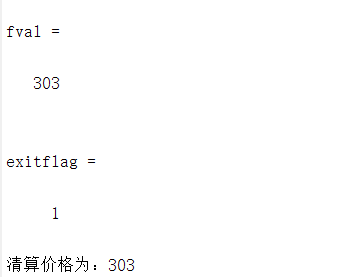
\includegraphics[width=0.5\textwidth]{result.png}
		\caption{result}
		\label{fig:fig1}
	\end{figure}
	
\end{document}